%% This is an article based on superfri.cls class file of
%% ``Supercomputing Frontiers and Innovations. An International Journal''
%% http://superfri.org/.

\documentclass{superfri}
\usepackage{graphicx}
\usepackage[hidelinks]{hyperref}

\usepackage{array}
\usepackage{todonotes}
\usepackage[capitalize]{cleveref}
\Crefname{lstlisting}{Listing}{Listings}
\usepackage{subcaption}
\usepackage{comment}
\usepackage{float}
\usepackage[utf8]{inputenc}
\usepackage{listings}
\usepackage{textcomp} %for upquote=true (straight quotes)
\definecolor{pblue}{rgb}{0.13,0.13,1}
\definecolor{pgreen}{rgb}{0,0.5,0}
\definecolor{pred}{rgb}{0.9,0,0}
\definecolor{pgrey}{rgb}{0.46,0.45,0.48}
\lstset{
    basicstyle=\ttfamily\footnotesize,
    numberstyle=\ttfamily\tiny,
    frame=single,
    numbers=left,
    numbersep=1em,
    xleftmargin=2em,
    language=XML, % to avoid type being blue
    breaklines=true,
    breakatwhitespace=true,
    postbreak=\hbox{$\hookrightarrow$ },
    showstringspaces=false,
    tabsize=2,
    commentstyle=\color{pgreen},
    keywordstyle=\color{pblue},
    stringstyle=\color{pred},
    moredelim=[il][\textcolor{pgrey}]{\[\]},
    moredelim=[is][\textcolor{pgrey}]{\%\%}{\%\%},
  columns=fullflexible,
    upquote=true
}

\newcommand{\jk}[1]{\todo[inline]{JK: #1}}
\newcommand{\lr}[1]{\textcolor{cyan}{LR: #1}}
\newcommand{\hh}[1]{\textcolor{blue}{HuangHua: #1}}
\newcommand{\bnl}[1]{\textcolor{green}{BNL: #1}}
\pagestyle{plain}

% ------------
\bibliographystyle{superfri}

\begin{document}

\author{Julian M. Kunkel\footnote{\label{uread}University of Reading, Reading, United Kingdom}\orcidID{0000-0002-6915-1179} \and Luciana R. Pedro\footnoteref{uread}\orcidID{0000-0001-8365-6264}
}

\title{Potential of I/O-Aware Workflows in Climate and Weather}

\maketitle{}

\begin{abstract}
The efficient, convenient, and robust execution of data-driven workflows and enhanced data management are key for productivity in scientific computing.
In HPC, the concerns of storage and computing are traditionally separated and optimised independently from each other and the needs of the end-to-end user. However, in complex workflows, this is becoming problematic. These problems are particularly acute in climate and weather workflows, which as well as become increasingly complex and exploiting deep storage hierarchies, can involve multiple data centres.

The key contributions of this paper are:
1) A sketch of a vision for an integrated data-driven approach, with a discussion of the associated challenges and implications, and 2) An architecture and roadmap consistent with this vision that would allow seamless integration into current climate and weather workflows as it utilises versions of existing tools (Cylc, XIOS, DDN IME, and ESDM).

The vision proposed here is built on the belief that workflows composed of data, computing, and communication-intensive tasks should drive interfaces and hardware configurations to best support the programming models.
When delivered, this work will increase the opportunity for smarter scheduling of computing by considering storage in heterogeneous storage systems.

\keywords{workflow, climate, weather, heterogeneous storage, data-driven}
\end{abstract}

% -----------------------------------------------------------------------

\section*{Introduction}
\label{sec:intro}

High-Performance Computing (HPC) harnesses the fastest available hardware components to enable the execution of tightly coupled applications from science and industry.
Typical use-cases include numerical simulation of physical systems and analysis of large-scale observational data.
In the domain of climate and weather, there is a considerable demand for the orchestration of ensembles of simulation models and the generation of data products.
A service such as the operational weather forecast workflow in Met Office writes around 200\,TB and reads around 600\,TB every day.
%For a typical Met Office Unified Model (UM) from the Coupled Model Intercomparison Project (CMIP) run, some %rough estimates of data volumes are:
%\begin{itemize}
%\item N96-ORCA1 -- 200Gb per model year
%\item N216-ORCA025 -- 700Gb per model year
%\end{itemize}
%Historical data spans over 170 years, generating 34Tb for low resolution and 119Tb for high resolution, while %projections will generate approximately half of this.
In total, at the Met Office, on average 1.5\,PB and 14\,PB are written and read per day, respectively, for all climate and weather forecasts across all HPC clusters.
%The above supports the view of how vital data management already is, and these numbers will grow with resolution and more ensembles.
%Existing climate experiments do ensemble experiments sequentially as few institutions have resources for parallel climate ensembles.
%That's an exascale use case requiring not only a big machine but the ability to schedule big jobs.
%\lr{I don't quite understand the numbers.}

Based on the needs of climate and weather researchers, the HPC community has developed a software ecosystem that supports scientists to execute their large-scale workflows.
While the current advances correspond to a big leap forward, many processes still require experts.
For example, porting a workflow from one system to another still requires adjusting runtime parameters of applications and deciding on how data is managed.

Since performance is of crucial importance to large-scale workflows, careful attention must be paid to exploit the system characteristics of the target computing centre.
For instance, a data-driven workflow may benefit from the explicit and simultaneous use of a locally heterogeneous set of computing and storage technologies.
This means that substantial changes may be required to a workflow to tailor it to a particular supercomputer environment in order to obtain the best performance.

%For example, porting a workflow from one system to another still requires adjusting runtime parameters of applications and deciding on how data is managed.}

Knowing the capabilities, interfaces, and performance characteristics of individual components are mandatory to make the best use of them.
As the complexity of systems expands and alternative storage and computing technologies provide unique characteristics, it becomes increasingly difficult even for experts to manually optimise the usage of resources in workflows. In many cases, modifications are not performed because: 1) They are labour intense: any change to the workflow requires careful validation which may not pay off for small scale runs; 2) It is a one-time explorative workflow and, 3) Users are not aware of the potential of the complex system.

In this paper, we illustrate how knowing the Input/Output (I/O) characteristics of workflow tasks and overall experimental design helps to optimise the execution of climate and weather workflows.
Exploiting this information automatically may increase the performance, throughput and cost-efficiency of the systems, providing an incentive to users and data-centres that cannot be neglected any longer.
Our approach intends to reduce the burden on researchers and, at the same time, optimise the decisions about jobs running on HPC systems.

This paper is structured as follows.
First, we describe the software stack involved in executing workflows in climate and weather in \Cref{sec:workflows}.
Related work in heterogeneous storage environments and solutions for workflow processing are presented in \Cref{sec:art}.
Next, the vision for including knowledge about data requirements and characteristics is sketched in \Cref{sec:vision} outlining the potential benefit the automatic exploitation might bring.
Our design, based on existing components in climate and weather, is described in \Cref{sec:design}.
The paper is concluded in \Cref{sec:conclusions}.

\section{Workflows in Climate/Weather}
\label{sec:workflows}

In this section, we describe how workflows are executed in a typical software stack and the typical hardware and software environment involved in running an application.

\subsection{Cylc}

Cylc~\cite{8675433} is in charge of executing and monitoring cyclic workflows in which each step is submitted to the batch scheduler of a data centre.
%Cylc development began in 2008 in response to deficiencies of existing NWP workflow schedulers related to the creation of a single never-ending workflow rather than a never-ending sequence of single-cycle workflows.
%With the current techniques, the evolution of the workflow could be a significant impediment
With Cylc, tasks from multiple cycles may be able to run concurrently without violating dependencies, preventing the issue of delays that cause one cycle to run into another.
Cylc was written in Python and built around a new scheduling algorithm that can manage infinite workflows of cycling tasks without a sequential cycle loop.
At any point during workflow execution, only the dependence between the individual tasks matters, regardless of their particular cycle points.
The information Cylc uses to control a given workflow is the task dependency.
In a script file, the developers define, for each task, the parallelism settings and where the data is to be stored.
%Decisions about storage must take into consideration the system architecture and the relevance of heterogeneous infrastructure in which the workflow will run.

\fig{width=0.8\columnwidth}{pic/cylc1}{Example of a Cylc workflow with its configuration file}

Consider the Cylc workflow for a toy monthly cycling workflow in \cref{pic/cylc1}.
In this workflow, an atmospheric model (labelled as \texttt{model} in the figure) simulates the physics from a current state to predict the future, for example, a month later.
In climate research, this process is repeated in the model to simulate years into the future.
% Once the simulation of any month is computed, this task completes and implicitly the data for this month becomes available and can now be analysed.
Once the simulation of any month is computed, the data for this month becomes available and can now be analysed.
In this workflow, the task \texttt{model} is followed by tasks postprocessing (\texttt{post}), forecast verification (\texttt{ver}), and product generation (\texttt{prod}), all specified as a workflow in a Cylc configuration file (\texttt{flow.cylc}).

\subsection{Workflow Execution}

While Cylc is directing the execution of workflows, several components are presented in the implementation.
The software stack involved in a general workflow is depicted in \cref{pic/stages}.
%As a preliminary, the user has to specify a configuration representing the Cylc workflow and provide scripts for the individual tasks/applications to be executed.
In the following, each stage of the execution is further described.

\fig{width=0.7\textwidth}{pic/stages}{Software stack and stages of execution}

\begin{enumerate}

  \item \textbf{Scientist} specifies the workflow and provides a command or a script for each task.
  As part of the Cylc configuration, the command(s) to be run, any environment variables used by these application(s), and any workload manager directives.
  After that, the user enacts Cylc to start the workflow.

  \item \textbf{Cylc} parses the workflow configuration file, generates tasks dependencies, defines a schedule for the execution, and monitors the progress of the workflow.
  Once a task can be executed (dependencies are fulfilled), the workflow engine submits a \textit{job script} for the workload manager with the required metadata that will run the Cylc task script.

  \item \textbf{Workload Manager} such as Slurm~\cite{Jette02slurm:simple} is responsible for allocating compute resources to a batch job and performing the job scheduling.
%  In our case, it now queues the job that represents the Cylc task and plans its execution, considering the scheduling policy of the data centre.
  The selected tool queues the job that represents the Cylc task and plans its execution, considering the scheduling policy of the data centre.
  Once the job is scheduled to be dispatched, i.e., resources are available, and the job priority is the highest, it is started on the supercomputer.

%  \item \textbf{Job} provides the environment with the resources it runs the user-provided script on one of the nodes allocated for the job.
%  The job sets environment variables containing information about the environment of the batch job, e.g., the compute nodes allocated, and then enacts the Cylc provided script on one node.

  \item \textbf{Job} provides the environment with the resources and it runs the user-provided program or script on one of the nodes allocated for it.
  Local variables containing information about the environment of the batch job, e.g., the compute nodes allocated, and then enacts the Cylc provided script on one node.

  \item \textbf{Script} executes the commands with one or multiple (potentially parallel) applications to run sequentially.
  During the creation of the script, Cylc has included variables that describe the task in the workflow.
  The information is typically fed into the application(s) representing the task, and so defines the storage location.
  The user script may use commands to generate filenames considering the cycle and may store data in a workflow-specific shared directory.

  \item \textbf{Application} is executed taking the filenames set by the script.
\end{enumerate}

\subsection{I/O Stack of a Parallel Application}

% \fig{width=0.2\textwidth}{pic/layers-xios}{I/O path for an MPI-parallel application}

\begin{figure}[b]
    \begin{minipage}{.42\linewidth}
        \centering
        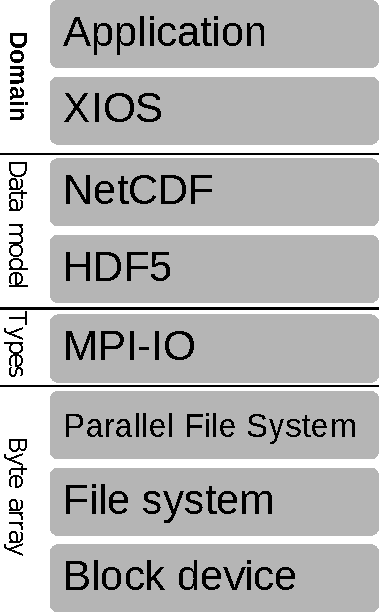
\includegraphics[width=0.42\textwidth]{pic/layers-xios}
        \subcaption{I/O path for an MPI-parallel application}\label{pic/layers-xios}
    \end{minipage}
    \begin{minipage}{.58\linewidth}
        \centering
        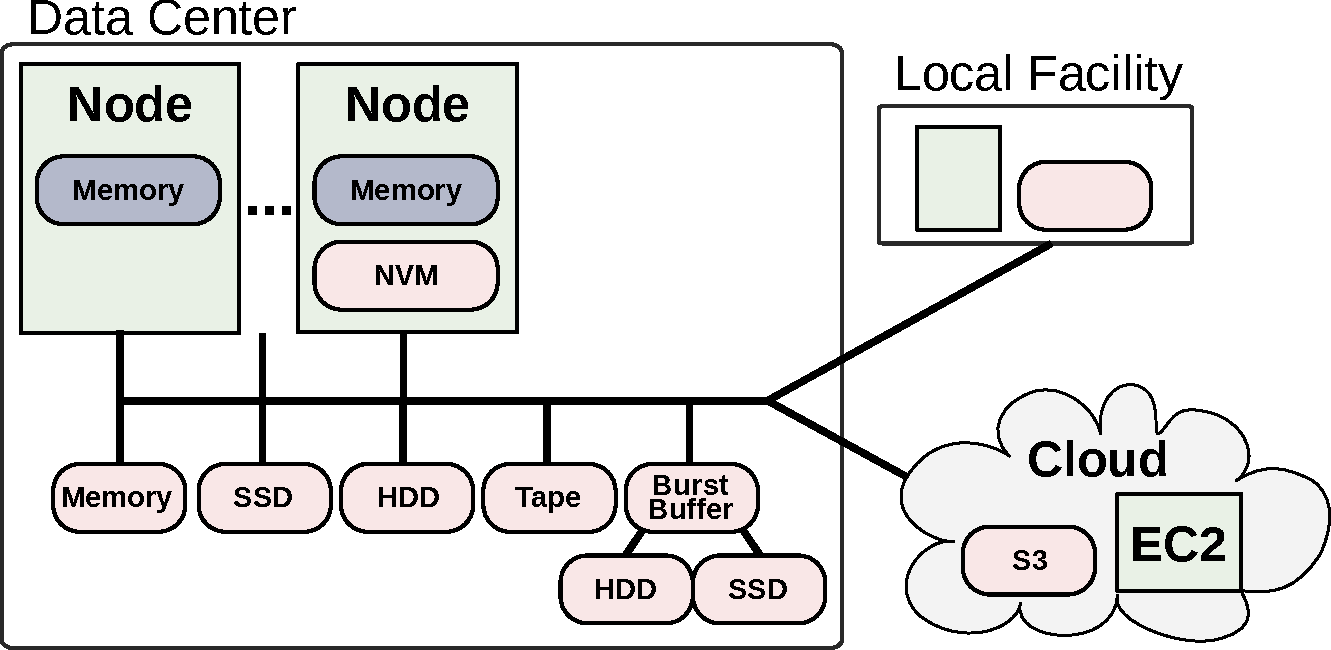
\includegraphics[width=1\textwidth]{pic/system}
        \subcaption{Example of an heterogeneous HPC landscape}\label{pic/system}
    \end{minipage}
    \vspace{5pt}
    \caption{Typical hardware and software environment for applications}
    \label{fig:34}
\end{figure}

% In our example, we assume the application is parallelised for performance reasons using MPI.
% Not just for performance reasons, it's about making enough memory too, so removed qualification.

Climate applications may have complex I/O stacks, as can be seen in \cref{pic/layers-xios}.
In this case, we assume the application uses XIOS~\cite{xios}, which is providing domain-specific semantics to climate and weather.
It may gather data from individual fields distributed across the machine (exploiting MPI for parallelism) and then uses NetCDF4~\cite{netcdf} to store data as a file.
Under the hood, NetCDF4 uses the HDF5 API with its file format.
Internally, HDF5 uses MPI and its data types to specify the nature of the data stored.
Finally, data is stored on a parallel file system like Lustre which, on the server-side, stores data in a local file system on block devices such as SSDs and HDDs.

Different applications involved in a workflow may use different I/O stacks to store their outputs.
Naturally, the application which uses previously generated data as its inputs must use a compatible API to read the specific data format.
In \cref{pic/layers-xios}, for example, XIOS may perform parallel I/O via the NetCDF4 API, allowing subsequent processes to read data directly using NetCDF4.
Within the ESiWACE project\footnote{\url{https://www.esiwace.eu/}}, we are developing the Earth System Data Middleware (ESDM)\cite{esdm} to allow applications with this kind of software stack to exploit heterogeneous storage resources in a data centre.
The goal of ESDM is to provide parallel I/O for parallel applications, with advanced features to optimise subsequent read accesses.
Implemented with a standalone API, it also provides NetCDF integration allowing usage in existing applications.
Hence, in \cref{pic/layers-xios}, the HDF5 layer can be replaced with ESDM.

\subsection{Data Center Infrastructure}

Data centres are providing an infrastructure consisting of computing and storage devices with different characteristics, making them more efficient for specific tasks and satisfying the needs of different workflows.
Take, for example, the supercomputer Mistral at DKRZ, that consists of 3,321 nodes\footnote{\url{https://www.dkrz.de/up/systems/mistral}} and offers two types of compute nodes equipped with different CPUs and GPU nodes.
Each node has an SSD for local storage, and DKRZ has additionally two shared Lustre file systems with different performance characteristics.
Individual users and projects are mapped to one file system explicitly, and users can access it with work or scratch semantics.
While data is kept on the work file system indefinitely, available space is limited by a quota.
The scratch file system allows storing more data, but data is automatically purged after some time.

Future centres are expected to have even more heterogeneity. A variety of accelerators (GPU, TPU, FPGAs), active storage, in-memory, and in-network computing technologies will provide storage and processing capabilities.
\cref{pic/system} shows such a system with a focus on computation and storage.
Some of these technologies might be local to specific compute nodes or globally available.
Depending on the need, the storage characteristics range from predictable low-latency (in-memory storage, NVMe) to online storage (SSD, HDD), and cheap storage for long-term archival (tape).
% Burst buffer solutions provide a tiered storage system that aims to exploit a storage hierarchy. % (\url{https://www.ddn.com/products/ime-flash-native-data-cache/})
The tasks within any given workflow could benefit from utilising different combinations of storage and computing infrastructure.

% \fig{width=0.6\columnwidth}{pic/system}{Example of an heterogeneous HPC landscape}

\subsection{Data Management}
\label{sec:datamanagement}

Usually, the scripts representing tasks define how the data is placed on the available storage system.
What happens in many current workflows is that they ignore the benefits of using multiple file systems concurrently and the data locality between tasks to colocating them.
On top of that, in the current state-of-the-art, scientists optimise the available storage resources intuitively and compile the information about this decision-making process manually.

If a user knows the workflow and the system characteristics, s/he can optimise data placement decisions.
Consider, for instance, the situation where each computing node has access to three file systems: a fast \texttt{scratch} file system on which data may reside only for a week, a slower \texttt{work} file system, and a \texttt{local} file system.
Most current workflows utilise \texttt{work} and \texttt{scratch} systems.
When a task is set to run, the corresponding dataset would be moved from \texttt{work} to \texttt{scratch}, processed, and the resulting dataset would be transferred back to \texttt{work}.
If the \texttt{scratch} filesystem reaches its capacity, the dataset would be moved back to \texttt{work}, and the task would continue running until it is finished, which might be inefficient. %\texttt{local} is not used.
In this situation, there are many obvious opportunities to utilise data migration to optimise performance, and other criteria (e.g., costs).
However, with a multitude of file systems that differ at each data centre, such optimisations would be difficult to achieve manually by users.
Policy-driven systems and burst-buffers perform such optimisations automatically to some extent. However, as they lack information about the workflow, they cannot optimise workflows perfectly.

\section{State-of-the-Art}
\label{sec:art}

Related work can be categorised into:
1) Technology that exploits heterogeneous storage environments and supports user-directed policies and
2) Solutions for workflow processing.

\textbf{Technology.}
Manual tiering requires the user or application to control the data placement, i.e., storing data typically in the form of files on a particular storage system and, usually, moving data between storage by scripts.
One limitation of such an approach is that decisions about how data are mapped and packaged into files are made by the producing application, and cannot be changed without manual intervention by a downstream application.

Burst buffer solutions provide a tiered storage system that aims to exploit a storage hierarchy.
They can be integrated into hardware capabilities such as DDN IME~\cite{BODIAIFSFI19} or simple software solutions.
A policy system, e.g., deployed on a burst buffer~\cite{RomanusRP15}, aims to simplify the data movement for the user, but typically migrates objects in the coarse granularity of files.
File systems and data management software such as IBM Spectrum Scale~\cite{SchmuckH02}, HPSS~\cite{528214}, BeeGFS~\cite{beegfs}, and Lustre~\cite{abs-1903-01955} (e.g., using the progressive file layouts feature) provide hierarchical storage management allowing to store data on different storage technology according to administrator-provided policies.
However, the semantic information that can be used by this type of system to make decisions is limited, e.g., data location, file extension, age of the file, etc.

The storage community had also adjusted various higher-level software to support storage tiering on top of several storage systems. For instance, ADIOS provides in-memory staging that had been exploited by a variety of applications~\cite{slawinska2013maya}.
Hermes~\cite{kougkas2020acceleration} provides a multi-tiered I/O buffering system with pre-fetcher that provides several data placement policies.
iRODS~\cite{rajasekar2010irods} is a rule-oriented data system that allows scientists to organise data into shareable collections and provides several patterns for workflows considering data locality and data migration/replication.
% and provide metadata such as the data life cycle.
Finally, there have also been extensions to batch schedulers to perform data staging for utilising node-local storage, for example, NORNS~\cite{miranda2019norns} as an extension to Slurm.

\smallskip

\textbf{Workflows. }
A good overview of the flavours of Scientific Workflow Management Systems (SWfMS) and their application to data-intensive workflows is given in \cite{liu2015survey}.
The article states that SWfMS should enable the parallel execution of data-intensive scientific workflows and exploit large amounts of distributed resources.
%"An abstract scientific workflow is defined by the functionality of each activity (or sub-workflow) and data dependencies between activities (or sub-workflows)"
Existing solutions recognise challenges in data variety (formats of the input data), opportunities to optimise the schedule by moving code to data, allow specifying the data dependencies for tasks, and they even may consider the capacity of the available data storage.
The execution engine Dryad~\cite{isard2007dryad}, for example, allows transferring data between tasks via files or directly using TCP connections and attempts to schedule tasks on the same nodes or racks.
Swift/T is a scripting language for describing dataflow processing allowing to execute ensembles of applications~\cite{ozik2016desktop}.
Recent improvements aim to migrate data to a local cache allowing to exploit locality.
For instance, in \cite{dai2018cross}, information about locality is proposed to be stored in extended attributes.
In \cite{TUIBIHWLSC19}, an approach was presented to monitor and analyse I/O behaviour of HPC workflows.

Various early research in grid workflows and lately cloud use cases attempts to maximise data locality in that respect.
Economic factors (including storage costs) for workflow execution are discussed in \cite{alkhanak2016cost}.
In \cite{deelman2019role}, the authors discuss the role of Machine Learning (ML) for workflow execution and elaborate a general potential for resource provisionings such as optimisation of runtime parameters, data movements, and hierarchical storage.
In \cite{subedi2019leveraging}, an ML model that stages data for in-situ analysis by exploiting the access patterns is introduced.


%TRIO: Burst Buffer Based I/O Orchestration. In: 2015 IEEE International conference on cluster computing, Chicago, IL, USA, 8–11 September 2015, pp. 194–203. Washington, DC: IEEE.
%Chervenak, A.L., Smith, D.E., Chen, W., Deelman, E.:
%Integrating policy with scientific workflow management
%for data-intensive applications. In: Supercomputing (SC)
%Companion: High-Performance Computing, Networking
%Storage and Analysis, pp. 140–149 (2012)

% https://www.sciencedirect.com/science/article/pii/S0167739X14002519
%Workflow engine for cloud \cite{pandey2011workflow}
%staging data to an available location just somehow.
%"storage service provides a temporary repository for application files that is, input files that are required for task execution, and output files that are the result of execution.""

Workflow systems can also be utilised specifically to reproduce scientific results, i.e., recompute the results.
Those scalable workflow solutions typically utilise a container solution to allow execution in an arbitrary software environment.
Popper~\cite{jimenez2017popper}, Snakemake~\cite{bts480}, and Nextflow~\cite{Nextflow} provide a language to specify workflows and to execute them.
Snakemake is interesting as it supports to define and infer input and output filenames.

While various aspects of our vision have been addressed individually by related work for different domains, the high level of abstraction that we aim for and the potential it unleashes goes beyond the capabilities of existing approaches.

\section{Vision for I/O-Aware Workflows}
\label{sec:vision}

Nowadays, in order to run a job in an HPC environment efficiently, researchers have to develop profound knowledge, not only about their workflow, which is expected, but also about decisions regarding storage, communication, computing, and considerations regarding cost-efficiency of those operations.
However, applied scientists should not spend much time understanding hardware characteristics and operative knowledge of running a data centre, but using their knowledge to develop their work and just collect and analyse the results.

We aim for achieving an automatic and dynamic mapping of I/O resources to workflows.
Once we have an automated decision about where the job will run and how the storage will be managed, scientists can then reuse their workflow specification on any system without further modification and even without previous knowledge about the system architecture.

There are several approaches to implement the technology for the vision proposed in this work, and changes are needed in the software components to realise it.
In \Cref{sec:design}, we will discuss a specific design for our transitional roadmap considering climate and weather workflows and tools scientists from this field already use in their routine research.

Our vision for I/O-aware workflows requires two additional pieces of information.
Firstly, the user must augment the workflow description with information about I/O requirements and explicitly annotate dependencies to datasets.
Secondly, details about the storage architecture must be available.

\subsection{System Information}

While many optimisations are possible once an abstraction is in place, the improvements we discuss here are related to the life cycle of datasets and the placement of such datasets into specific storage according to system performance characteristics and the workflow specification.
To achieve that, the system information shall comprise of all available storage systems, the system topology, and details of each of the required components.
Simplified and complex models of the components can be included to approximate expected performance for specific I/O patterns.
It is expected that the data centre (or expert users) can create such a configuration file, e.g., by using vendor-provided information or by executing benchmarks.
With this information, a scheduler can make the initial data placement, transformation, and migration decisions for individual datasets during their life cycle.
This separation of concerns allows us to abstract from the workflow what is essential and what a system should optimise to ensure smart usage of the available resources.

\subsection{Extended Workflow Description}

In general, climate and weather workflows allow specifying tasks and the dependencies among them.
We aim to enhance the current information with characteristics for input and output, i.e., the datasets.
An example workflow with \texttt{N} cycles containing input datasets and (intermediate) products is illustrated in \cref{pic/workflow-s3-n}.
Round nodes represent tasks, squared nodes represent data, and arrows indicate dependencies.
In the example, Task\,1 needs two datasets to perform its work, produces Product\,1, and it directly communicates with Task\,2.
For each new cycle, the \texttt{checkpoint} from the previous cycle (Product\,1) is used as input to starting the next cycle.
Most of the workflow can run automatically, except for the manual quality control of the products and the final data usage of Product\,3.
This last step represents the typical uncertainty of data reuse, i.e., it is unclear how Product\,3 will be used further.
In the approach proposed in this work, each task is annotated with the required input datasets and the generated products must include metadata such as data life cycle information, the value of data, and how long it should be kept.
The idea here is to embrace the concept that tasks dependencies are really imposed by datasets dependencies.

\fig{width=0.8\columnwidth}{pic/workflow-s3-n}{Example of a high-level workflow with tasks and data dependencies}

%The access to I/O information before the workflow runs can be used to optimise where jobs will be executed and how datasets will be stored during the workflow.
%This information today is static and manual, leaving open opportunities for automating and optimisations.
%Once we insert the datasets explicitly in the workflow, it is easier to see that many optimisations regarding storage can be made.

\subsection{Smarter I/O Scheduling}

The abstraction and automation of the I/O inside a workflow allow a runtime system to improve data placement and apply data reduction on heterogeneous storage systems.
Taking into consideration the architecture and workflow information, a smarter schedule can now be realised by exploiting the additional information.
Value and priority can influence fault-tolerance strategies and imply the quality of service for performance and availability.
Aspects like data reproducibility (can it be recomputed easily), type of the experiment (test, production), and runtime constraints for the overall and potential workflow could allow reducing costs and, hence, increasing scientific output.
Next, we outline the two core strategies and potential the proposed vision can bring to improve current workflows.
In the design proposed in this work (\cref{sec:design}), we will focus on the data placement strategy.

% \subsubsection{Data Placement}

\paragraph{Strategy: Data Placement.}

Data placement encompasses all data movement-related activities such as transfer, staging, replication, space allocation and de-allocation, registering and unregistering metadata, locating and retrieving data\footnote{https://www.igi-global.com/dictionary/data-aware-distributed-batch-scheduling/6782}.
The general idea is to host a dataset on the storage system that is most favourable in terms of performance, cost-effectiveness, availability for the access pattern observed in the workflow.
Here we are considering the optimisation of data locality, where locality is twofold, spatial and temporal on a variety of characteristics.
For optimising data placement, there are several approaches:%: \textbf{in-memory data}, \textbf{data allocation}, \textbf{data migration}, and \textbf{data replication}.

\begin{description}

\item[Data Allocation] is the assignment of a specific area of an available storage system to particular data.
In current workflows, the user usually has a script for each task defining the filenames with a prefix that places datasets generated by the same task into a specific storage\footnote{Complicated scripts would have allowed changing the storage type depending on the cycle. Still, it is a significant burden to the user.}.
Because there is one script responsible for generating the configuration, the decision in which directory the dataset will be stored is somewhat fixed.
Such configuration is done manually and with restricted information about the system architecture.
It would be interesting to explore storage options for the datasets and, e.g., having datasets from different cycles placed at different storage systems.
For instance, in \cref{pic/workflow-s3-n}, alternating the storage location for Product\,2 into two scratch file systems is something that would be a simple job for an I/O-aware scheduler.
However, currently, that implies providing scripts for that task and all tasks depending on the data with information about the different storage placement.
%Next, we exemplify three situations in which data placement can be optimised.

\item[Data Migration] is the process of transferring data from one storage system to another. Typically, it involves to delete the data, but this decision can be delayed to provide read access to multiple storage systems.
Data movement involves a significant overhead as data must be read on one storage and written to another, both in terms of latency and energy-efficient computing, hence needs to be considered carefully.
\cref{fig:lifecycle} introduces three possible life cycles for a specific dataset and explains how migrations can be done to improve datasets accessibility.
In \cref{fig:lifecycle1}, the dataset could be first stored on the \texttt{local} storage to avoid congestion on the \texttt{work} file system, then be migrated to \texttt{work} file system where subsequent tasks of the workflow may read it multiple times.
In the end, this dataset may be an intermediate product that can then be deleted.
In \cref{fig:lifecycle2}, the dataset is stored on the \texttt{scratch} file system immediately and accessed there.
%However, that would require subsequent tasks to be placed on the same node where data is now stored, and the last read access must happen before files on \texttt{scratch} are automatically removed.
However, the last read access must happen before files on \texttt{scratch} are automatically removed.
Alternatively, \cref{fig:lifecycle3} presents the case where the dataset is created on \texttt{work} by a task and it is copied to a \texttt{local} node.
This \texttt{local} node allows reading accesses of subsequent tasks which might be beneficial for small random accesses.
For the last two scenarios, subsequent tasks would have to be placed on the same node where previous data was stored.
%However, it would require that the subsequent tasks are placed on the same node where data is now stored.

\begin{figure}[b]
    \begin{minipage}{.33\linewidth}
        \centering
        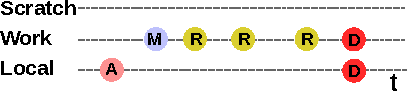
\includegraphics[width=0.9\columnwidth]{pic/lifecycle-1}
        \subcaption{Local and work file systems}\label{fig:lifecycle1}
    \end{minipage}
    \begin{minipage}{.33\linewidth}
        \centering
        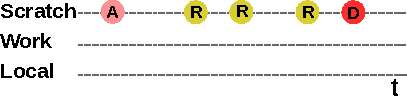
\includegraphics[width=0.9\columnwidth]{pic/lifecycle-2}
        \subcaption{Scratch file system only}\label{fig:lifecycle2}
    \end{minipage}
    \begin{minipage}{.33\linewidth}
        \centering
        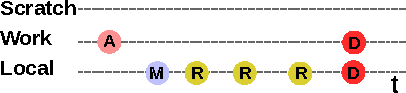
\includegraphics[width=0.9\columnwidth]{pic/lifecycle-3}
        \subcaption{Local and work file systems}\label{fig:lifecycle3}
    \end{minipage}
    \vspace{5pt}
    \caption{Alternative life cycles for mapping a dataset to storage and the operations: \textbf{A}llocation, \textbf{M}igration, \textbf{R}eading, and \textbf{D}eleting}
    \label{fig:lifecycle}
\end{figure}

\item[Data Replication] in computing involves sharing information to ensure consistency between redundant resources, such as software or hardware components, to improve reliability, fault-tolerance, or accessibility.
Data might be replicated by enabling the system to rerun parts of the workflow in case of a data loss.
In addition, the system may combine the replication of data by \textbf{transforming} the data into a different representation allowing to achieve better performance for a variety of access patterns.

\item[Direct-Coupling] replaces I/O by communicating data between subsequent steps of a workflow directly without storing intermediate data products on persistent storage.
As an example, in \cref{pic/workflow-s3-n}, the outcome of Task\,1 may be used directly by Task\,2.
To achieve some level of independence between producer and consumer, data may also be kept in memory and cached.
\end{description}


\paragraph{Strategy: Data Reduction.}

Data reduction reduces the amount of data stored.
We discuss here two potential optimisations: \textbf{data compression}, and \textbf{data recomputation}.

\begin{description}

\item[Data Compression] is the process of encoding information using fewer bits than the original representation.
Knowing the characteristics of data production and usage makes it simpler for scientists to annotate the required precision of data in those workflows.
The storage system can exploit such information by reducing the precision of data and automatically picking an appropriate compression algorithm.

\item[Data Recomputation] Climate/weather scientists are trading recomputation with space usage manually.
%, in the so-called field space-time trade-off that has been applied in Cryptanalysis for already forty years~\cite{1056220}.
By knowing how to rerun the workflow behind the data creation, a smarter storage system can automatically trade data availability for potential recomputation opportunities to optimise the cost-efficiency of the system.
Intermediate states could be rerun by utilising virtualisation and container technologies.
Consider \cref{pic/workflow-s3-n} again and that, at every \texttt{K} cycles of the workflow, the generated Product\,3 (from Cycle 1 to Cycle \texttt{K}) are used in a validation task, called here \texttt{check}.
From the workflow, we know that $P_3 C_1$\footnote{The $P_i C_j$ notation represents the Product\,$i$ generated in the Cycle $j$.} will be used to construct $P_3 C_2$ and then \texttt{check}.
This dataset would probably be stored somewhere, and it will not be used until the workflow reaches the \texttt{K}-th cycle.
One alternative is to delete it after it was first used and then recompute it when time is right.
The cost of doing that is storing \texttt{checkpoint} and then use it to reconstruct $P_3 C_1$.
If, for instance, $P_3 C_1$ is a large dataset, \texttt{checkpoint} is small, and computing time is short, it is easy to see that deleting and recomputing it may improve the costs of running the workflow.
%We need, then, information about datasets volume and computing time to be able to make an accurate decision.
%The bottom line here is: there are situations in which decisions are being made without considering all the available %information and possible scenarios.
This is just an example, and, currently, scientists perform those optimisations manually.
\end{description}

\subsection{Benefit}

The benefits of the proposed vision are:

\begin{description}

\item[Abstraction] The user does not have to know the architecture of the target system on which the workflow will run, removing the specialist from the decision-making process.

\item[Optimisation] The workflow will be optimised specifically for the available system infrastructure and extra information about the data.
In particular, by exposing the heterogeneous architecture, potentially runtime characteristics can be considered.
By using information about the value of data, policies for data management (storage resilience,  recomputation, replication, etc.) can be decided.

\item[Performance-portability] With both abstraction and optimisation, the user can specify the I/O requirements only once for the tasks of a specific workflow, and the I/O-aware workflow can now run with optimised data storage on any system without user intervention.
Even more, if the system characteristics change, e.g., it gets upgraded, an additional storage tier becomes available, or if storage degrades, the I/O-aware workflow could automatically adapt and make use of this new environment. % gain

\end{description}

\section{Design}
\label{sec:design}

This section describes our first approach to incrementally extend workflows for climate and weather that realises parts of our vision.
While individual components such as ESDM and Cylc exist, we have not implemented the described scheduler, yet.
To automatically make scheduling decisions, the software stack needs to:

\begin{enumerate}

\item Deliver information about dataset life cycle together with the workflow, and

\item Adapt the resulting workflow, individual scripts and application executions to consider the potential for data placement.
\end{enumerate}

\subsection{System Information}

ESDM is used as I/O middleware in the parallel application (with NetCDF or directly) and orchestrates the I/O according to a simplified ESDM configuration file (\texttt{esdm.conf}).
% The information about the system is provided using a simplified ESDM configuration file (\texttt{esdm.conf}) provided by the data centre (or expert users).
This file contains information about the available technology in the data centre, its I/O characteristics, and will be used to make decisions about how to prioritise I/O targets.
In the example presented in \Cref{lst:esdm.conf}, we have three storage targets: two global accessible file systems (\texttt{lustre01} and \texttt{lustre02}), and one local file system in \texttt{/tmp} that can be accessed via the POSIX backend.
Each of them comes with a lightweight performance model and the maximum size of data fragments.
The metadata section (Line 24) utilises here a POSIX interface to store the information about the ESDM objects. Internally, ESDM creates so-called containers and dataset objects to manage data fragments.

\begin{lstlisting}[caption = Example of an ESDM configuration file (\texttt{esdm.conf}), label=lst:esdm.conf]
"backends": [
    {"type": "POSIX", "id": "work1", "target": "/work/lustre01/projectX/",
        "performance-model" : {"latency" : 0.00001, "throughput" : 500000.0},
        "max-threads-per-node" : 8,
        "max-fragment-size" : 104857600,
        "max-global-threads" : 200,
        "accessibility" : "global"
    },
    {"type": "POSIX", "id": "work2", "target": "/work/lustre02/projectX/",
        "performance-model" : {"latency" : 0.00001, "throughput" : 200000.0},
        "max-threads-per-node" : 8,
        "max-fragment-size" : 104857600,
        "max-global-threads" : 200,
        "accessibility" : "global"
    },
    {"type": "POSIX", "id": "tmp", "target": "/tmp/esdm/",
        "performance-model" : {"latency" : 0.00001, "throughput" : 200.0},
        "max-threads-per-node" : 0,
        "max-fragment-size" : 10485760,
        "max-global-threads" : 0,
        "accessibility" : "local"
    }
],
"metadata": {"type": "POSIX",
        "id": "md",
        "target": "./metadata",
        "accessibility" : "global"
    }
\end{lstlisting}

%\hh{Here I have similar question: we need an extended and new configuration file, which includes characteristics of inputs/outputs dataset. As Julian said above, we can not added these items directly into Cylc configuration because Cylc wouldn't understand it. But you see, it's a burden to have another conf file. It is error-prune, and duplicated information may cause inconsistency. I propose to have these information added to the same Cylc configuration file, but in special comments. These comments will be omitted by Cylc, but they can be parsed by ESDM. This is similar for Doxygen comments in C/Java source file, or the leading line of a shell script, etc.}
%\jk{Good suggestion! That absolutely depends how a Cylc file is parsed and analysed. Keeping it separately gives us the most flexibility and parsing comments could lead to misinterpreting already existing comments and acting wrongly. Still to consider.}

%\hh{Other requirements of datasets may be: data block size/fragment size, 1-1 or N-1 access mode, IOPS intensive or throughput-intensive, etc. These will also be considered for data placement and migration.}
%\jk{Fragment size/data blocks are handled by ESDM automatically. The access mode and access pattern is something that we could consider to add. However, difficult for scientists to judge}

ESDM manages a pool of threads that should be created per compute node to achieve good performance and delegates the assignment of optimal block sizes to the storage backend.
The number of threads is defined in the configuration file.
As an example, based on the number of Object Storage Targets (OSTs) provided by both Lustre systems at DKRZ, performance tests already developed using ESDM~\cite{2019_3361225} shows that no more than 200 threads in total should be used to perform I/O to extract the best performance.
%; more degrade it.
To clarify the behaviour, ESDM distributes a single dataset across multiple storage devices depending on their characteristics.
Since ESDM also supports several (non-POSIX) storage backends, an application can utilise all available storage systems without any modifications to the code.

The configuration file is inquired by an application that utilises ESDM and steers the distribution of data during I/O.
While the current system information and performance model are based on latency and throughput only, it shows that automatic decision making can be made on behalf of the user.

\subsection{Extended Workflow Description}

The user now has to provide information about datasets required for input and the generated output for each workflow task in a separate file similarly to Cylc's workflow configuration file.
An example of an I/O-workflow configuration file (\texttt{io.cylc}) is shown in \Cref{lst:cylc}. In this file, information about Task\,1 is given by example, and we expect the extra information about all tasks in the same file. Ultimately, this could be integrated into the workflow specification file of Cylc.

\begin{lstlisting}[caption = External Cylc I/O-workflow configuration file (\texttt{io.cylc}), label=lst:cylc]
[Task 1]
  [[inputs]]
    topography = "/pool/input/app/config/topography.dat"
    checkpoint = "[Task 1].checkpoint$(CYCLE - 1)"
    init       = "/pool/input/app/config/init.dat"

  [[outputs]]
    [[[varA]]] # This is the name of the variable
      pattern = 1 day
      lifetime = 5 years
      type = product
      datatype = float
      size = 100 GB
      precision.absolute_tolerance = 0.1

    [[[checkpoint]]]
      pattern = $(CYCLE)
      lifetime = 7 days
      type = checkpoint
      datatype = float
      dimension = (100,100,100,50)

    [[[log]]]
      type = logfile
      datatype = text
      size = small
\end{lstlisting}

%In this example, the workflow file could define a cycle flexibly to be a month or a year according to the Cylc workflow file.
In this example, the \texttt{io.cylc} file could define a cycle flexibly to be a month or a year according to the \texttt{flow.cylc} file.
The notation is similar to the specification of Cylc workflows using a nested INI format.
For each task, inputs and outputs are defined.
In the input section, each entry specifies the virtual name that is used by ESDM as a filename inside NetCDF.
Line~3, for example, defines that the filename \texttt{topography} is mapped to a specific input file.
This dataset does not depend on any previous step of the workflow.
The next line specifies that the input filename \texttt{checkpoint} should be mapped to the output of Task~1 checkpoint dataset from the previous cycle (e.g., the checkpoint generated after completed the last year's output).
For the initial cycle, the checkpoint file will be empty, and the application will load the init data.
In the output section, the datasets are annotated with their characteristics more precisely.
For each variable, a pattern defining how frequently the data is output according to the workflow must be provided.
Most data is input and output in the periodicity of the cycle, except for \texttt{varA}, which is output per day regardless of the cycle.
Next, we formally define the expected annotations in all the fields expected in the I/O-workflow configuration file:

\begin{description}[itemsep=0pt]
  \item[Name] A basic name for the field/data generated. It is extended by a pattern defined in a variable (Lines: 8, 16, 23).

  \item[Pattern] The frequency the data is output (Lines: 9, 17).

  \item[Lifetime] How long the data must be retained on storage (if at all) (Lines: 10, 18).

  \item[Type] The class type of data, i.e., checkpoint, diagnostics, temporary (Lines: 11, 19, 24).

  \item[Datatype] The data type of the data (Lines: 12, 20, 25).

  \item[Size] An estimate of the data size\footnote{This field can be inferred if dimension and datatype are provided.} (Lines: 13, 26).

  \item[Dimension] The data dimension (Line: 21).

  \item[Accuracy] Characteristics quantifying the required level of data precision (Line: 14).

\end{description}

Note that the user may not be able to provide all required information.
This can be handled by assuming a default safe behaviour.
For instance, in the case of missing data precision, data should be retained in original form.
Knowing the dimension or size a priori might be difficult for scientists, e.g., the log file size is unclear.
In this case, the user may insert relevant information like small or big, reflecting that any information is better than no information at all.
In future, we will explore how to automatically infer the output volume from the input or by using monitoring.
By allowing to run using an empty I/O workflow specification and monitoring I/O accesses for one cycle, we can propose an I/O description to the user to simplify the specification.

\subsection{Smarter I/O Scheduling}

From the list of opportunities, we realise data placement and migration in a heterogeneous (multi-storage) environment.
These goals will be achieved via the proposed I/O-aware scheduler, called here EIOS (ESDM I/O Scheduler).
EIOS will make the schedule considering Cylc workflow, and ESDM provided system characteristics.
Components of it are involved in different steps of the workflow and the I/O path.

While Cylc schedules the workflow, EIOS can provide hints about colocating tasks which provide the opportunity for keeping data in local storage.
Decisions about data locality will not be made for a whole (and potentially big) workflow.
Instead, the system will make decisions by looking ahead to several steps of the workflow, allowing reacting to the observed dynamics of the execution.
We utilise DDN's IME API to pin data in IME and to trigger migrations between IME and a storage backend explicitly.

Ultimately, when a user-script runs, the information about the intended I/O schedule is communicated from EIOS through a modified filename, which is then used by the ESDM-aware application to determine the data placement.

\subsection{Modified Workflow Execution}

The steps to execute a workflow enriched with I/O information and perform smarter scheduling is depicted in \cref{pic/stages-io}.
The suggested alterations can be seen in boxes pointed by red arrows, and the remaining components are the current state-of-the-art for workflows in climate and weather from \cref{pic/stages}.
In the following, we describe the modifications we propose in this vision paper for each component involved in the software stack.

\fig{width=0.7\columnwidth}{pic/stages-io}{Software stack and stages of execution with the I/O-aware scheduler (EIOS)}

\begin{enumerate}

  \item \textbf{Scientist} The user now has to provide an additional file that covers the I/O information for each task and slight changes have to be made to the current scripts.

  \item \textbf{Cylc} EIOS is invoked by Cylc to identify potential optimisations in the schedule before generating the Slurm script.

  \item \textbf{\color{red}{EIOS}} The ESDM I/O Scheduler reads the information about the workflow (\texttt{flow.cylc} and \texttt{io.cylc} configuration files) and acts depending on the stage of the execution.
  EIOS consists of several subcomponents:
    \begin{itemize}

      \item The high-level scheduler that interfaces with Cylc.

      \item A tool to generate pseudo filenames used by the ESDM-aware applications.

      \item A data management service (not shown in the figure) that migrate and purge data at the end of the life cycle.
    \end{itemize}
  EIOS components use knowledge about the system by parsing the \texttt{esdm.conf} file.
  EIOS may decide that subsequent jobs shall be placed on the same node, reorder the execution of some jobs, and provide information for conducting data migration.

  \item \textbf{Slurm}
  Cylc may now have added an optimisation identified by EIOS which is now handled by a modified Slurm.
  Also, if migrations have to be performed, Slurm will administer them according to the specification in the job script.

  \item \textbf{Job}
  A job might run on the same node as a previous job to utilise local storage.
  %\bnl{Any interesting that needs this performance is running on dozens if not hundreds of nodes}

  \item \textbf{Script}
  Filenames are now generated by a replacement command that calls EIOS to create a pseudo filename.
  This filename will encode additional information for ESDM about how to prioritise data placement according to data access.

  \item \textbf{Application}
  The application may either use XIOS, NetCDF with ESDM support or ESDM directly to access datasets.
  Hence, in \cref{pic/layers-xios}, the HDF5 layer is replaced with ESDM.
  ESDM loads the \texttt{esdm.conf} file that contains the information about the available storage backends and their characteristics.
  ESDM extracts the long-term schedule information from the generated pseudo filenames and employs it during the I/O scheduling to optimise the storage considering data locality between tasks.
  Basically, ESDM can now change the priorities for data placement of the different storage locations that would normally be encoded in its configuration file.
\end{enumerate}

\section{Conclusions}
\label{sec:conclusions}

In the domain of climate and weather, organising the data placement on storage tiers is performed by the users or via policies, often leading to suboptimal decisions.
Additionally, the manual optimisation and hard-coding of storage locations is non-portable and an error-prone task.
We believe users must be able to express their workflows abstractly.
By increasing the abstraction level for scientists, not only tedious manual optimisation could be automatised, but also strategies for data placement and data reduction can be harnessed.
With knowledge about the data pattern, the runtime system could generate optimised execution plans and monitor their execution.
In this work, we describe the general vision and a specific design for the software stack in the domain in climate and weather that we work on in the ESiWACE project.
The proposed changes increase the opportunity for smarter scheduling of storage in heterogeneous storage environments by considering the characteristics of data and system architecture in a workflow.

\section*{Acknowledgements}

\small
This project is funded by the European Union's Horizon 2020 research and innovation programme under grant agreement No. 823988.
We thank our collaborators Bryan Lawrence, Glenn Greed, David Matthews, and Hua Huang for their input to this paper.

\openaccess

\bibliography{paper}

\end{document}

Machine Learning has been proven effective in replacing human-beings, and it may also adapt the workflow dynamically in case of unexpected situations (the system is down, nodes are unresponsive, etc.). (ref)

From the recorded I/O accesses, we analyse the I/O patterns and dependencies associated with it to generate the configuration file.

Potentially, EIOS may generate an \texttt{esdm.conf} file for the specific application to adjust the mapping of data to available storage targets.

In particular, a system could store data that is of low value or cheap to reproduce on storage with little redundancy or trade storage space by the need to recompute data products.

This scenario was developed to exemplify some of the potential optimisations we envision about \textbf{data placement}, \textbf{migration}, and \textbf{recomputation} in a heterogeneous storage environment.

The user-specific storage locations are a viable option to run a workflow.

The user might even have analysed various scenarios, such as depicted in Section \ref{sec:datamanagement}.

Assuming the user can provide extra information in advance, ESDM can interact in the process before the user gives the data to the Cylc tool, using the gathered information to construct a tentative optimised workflow.

Here, we focus on utilising a heterogeneous storage environment.

Once we have access to the data pattern, the whole workflow can be improved by trading storage space by the need to recompute data products.

With the right level of abstraction in place, potential data optimisations are unleashed in a heterogeneous storage system according to its characteristics and workflow specification.

Exploiting the value and importance of data could improve the placement decisions on heterogeneous storage systems.

Data systems usually do not respect, or have knowledge of, the importance of their inherent data.

%\hh{I like this idea of machine learning in storage system. A lot of analysis has been done on relation of I/O pattern and storage performance. But how to know the I/O pattern, data pattern in advance? Machine Learning can be used to find pattern. These patterns can then be used to schedule storage resources, data placement, data staging/migration, etc. These pattern can be gradually learned from running cycles of workflows over time, such that policies can evolve to have better performance when more and more cycles of workflow complete. }

CYLC_SUITE_SHARE_DIR
Typically the data generated by cylc workflows is stored in the “share” directory which is referenced by an environment variable rather than a command:
https://cylc.github.io/doc/built-sphinx/suite-config.html#suite-share-directories
